\documentclass{article}
\usepackage[utf8]{inputenc}
\usepackage[T1]{fontenc}
\usepackage[francais]{babel}
\usepackage{minted}
\usepackage{uqac}

%<----------->Meta-Data<----------->

\title{Premier Travail}
\author{Tristan MOLIN\\Florian FICHANT\\Martin LOCQUEVILLE}
\codep{}
\discipline{8INF914 - Visualisation Analytique}
\projet{Etude des algorithmes de dessin d'arbres \\ Travail de session \\ Rapport}
\date{\today}

%<--------------------------------->

\begin{document}

\maketitle

\tableofcontents

\newpage

\mainmatter

\section{Introduction}

L'objectif de notre projet est de parvenir à implémenter en \emph{Python}, au sein de l'outil d'étude de graphe \emph{Tulip}, un algorithme de dessin d'arbre, le plus optimal possible. Pour ce faire, nous avons recueilli et analysé les travaux de recherche dans quatre articles.

Ces articles avaient également comme problématique l'optimisation de dessin de graphe. Chacun d'eux cherchant à optimiser l'implémentation d'un algorithme de dessin d'arbre en prenant en compte les travaux de leurs prédécesseurs (Nous avons pris soin de noter les références de ces articles en fin de rapport).

Suite à l'étude de ces articles, nous allons premièrement implémenter les algorithmes résultant des travaux des auteurs de nos quatre articles de référence. C'est après cela que nous allons écrire de manière optimisée et implémenter notre solution algorithmique en \emph{Python}, en utilisant la bibliothèque \emph{Tulip}.

Pour finir, nous allons étudier plus en détail nos algorithmes à l'aide de jeux de données, permettant de voir ainsi s'ils répondent bien à leur objectif, s'ils peuvent éventuellement être améliorés au niveau du temps d'exécution, de l'écriture du code, etc.


\newpage
\section{Étude préliminaire des articles}

Ayant relevé une continuité chronologique, dans la mesure où les auteurs reprennent les travaux des précédents articles, notre étude des articles gardera cet ordre chronologique.

Avant d'entrer dans l'étude des algorithmes, il est important de définir les caractéristiques principales de ces graphes. Un arbre, tel que défini dans notre premier article \cite{article79}, est un graphe plan dans lequel aucune arête ne se croise, chaque n\oe{}ud du graphe comprend un unique prédécesseur (à l'exception du n\oe{}ud racine: \emph{Root}), un n\oe{}ud ne peut se trouver plus proche du \emph{Root} que ses n\oe{}uds parents, le dernier n\oe{}ud d'une branche (n\oe{}ud qui n'a pas de fils) est appelé feuille. La dernière caractéristique de base d'un arbre est l'alignement de ses n\oe{}uds, les n\oe{}uds d’une même hauteur doivent être sur la même ligne de sorte que toutes les hauteurs soient sur des lignes parallèles (cette dernière propriété est noté dans l'article \cite{article79}: \emph{Esthétique 1}).

Maintenant que notre arbre de base est défini, nous pouvons nous intéresser aux problématiques des articles concernant l'implémentation d'algorithmes (voir ci-dessous nos propriétés de base appliquées à un arbre).

\vfill
\begin{figure}[h]
		\begin{center}
			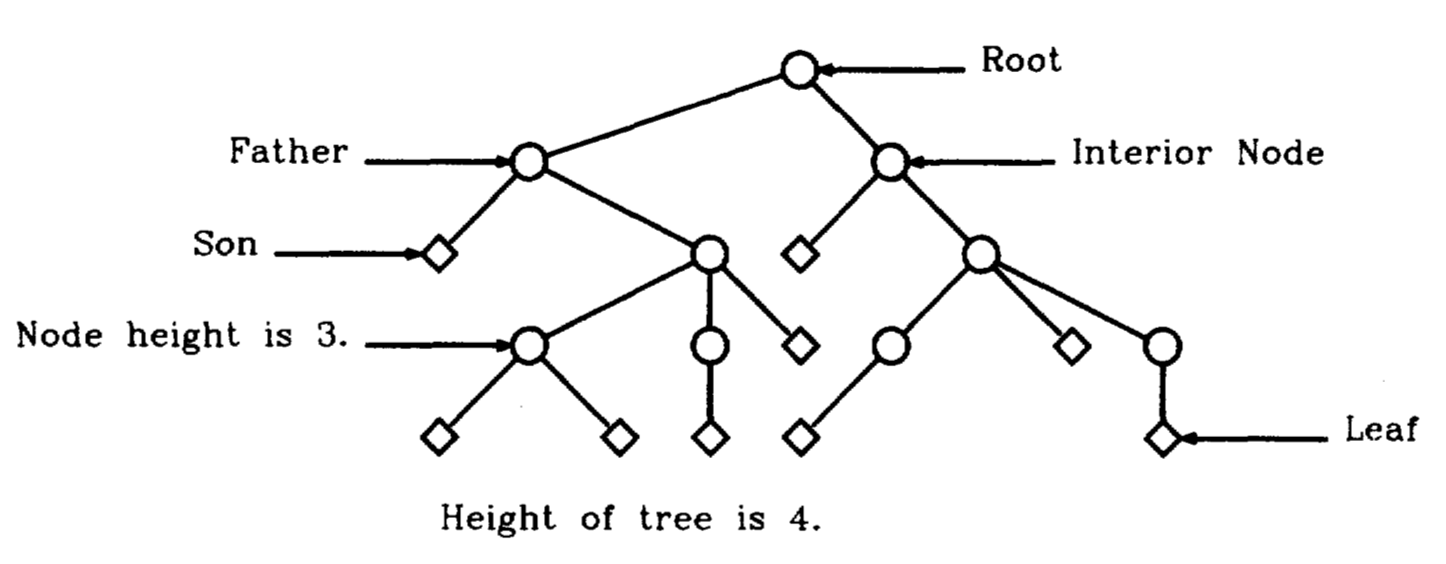
\includegraphics[scale=0.4]{arbre.png}
		\end{center}
	\caption{Exemple d'un arbre d'après nos premières propriétés. \cite{article79}}
  \label{fig:arbre}
\end{figure}
\vfill

\newpage
  \subsection{\emph{Tidy Drawings of Trees}}

  Les auteurs de l'article se sont penchés sur l'optimisation de dessin d'arbre. Dans un soucis d'espace sur lequel représenter les graphes, ils ont posé la problématique suivante (\emph{Limite Physique 1}):  la largeur de l’arbre doit être la plus petite possible (la hauteur est fixée par l’arbre). Pour rappel, la hauteur d'un n\oe{}ud correspond au nombre de branches entre lui et le \emph{Root} (cf: Figure \ref{fig:arbre} page \pageref{fig:arbre}).
    \subsubsection{A Naive Tree Drawer}

    Le premier algorithme (\emph{Algorithme 1}) de dessin d'arbre décrit par cet article est \emph{l'algorithme d'arbre naïf}. Il a comme objectif de répondre à la \emph{Limite Physique 1} en optimisant l'espace du graphe.

    Il prend en entrée un arbre, tel que nous l'avons défini plus haut, ainsi que la hauteur de cette arbre et retourne en sortie le même arbre dans lequel la position des n\oe{}uds a changé pour faire en sorte que l'arbre ait la largeur la plus étroite possible.

    Le fonctionnement de cet algorithme comprend une variable qui compte la prochaine coordonnée en $x$ de libre, pour y placer le prochain n\oe{}ud. Pour ce qui est de la coordonnée en $y$, elle correspond à la hauteur du n\oe{}ud dans l'arbre qui a été donnée en paramètre d'entrée de l'algorithme, de cette manière, on respecte toujours l'\emph{Esthétique 1}.

    \vfill
    \begin{figure}[h]
    		\begin{center}
    			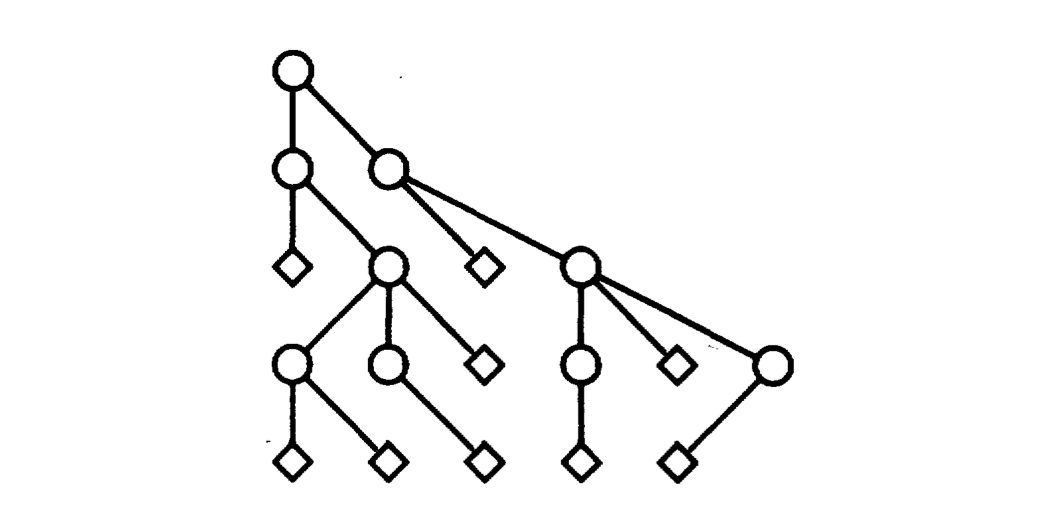
\includegraphics[scale=0.4]{arbreNaif.png}
    		\end{center}
    	\caption{Notre premier arbre modifié par l'\emph{Algorithme 1}. \cite{article79}}
      \label{fig:arbreNaif}
    \end{figure}
    \vfill

    \subsubsection{Binary Tree Drawings}

    L'algorithme que nous venons de voir est efficace, mais un problème se présente lorsque nous souhaitons faire apparaitre des labels sur les n\oe{}uds. Nous en venons maintenant à un algorithme qui nous permet de prendre en compte l'affichage de label sur notre graphe. Il a été conçu pour les arbres binaires (arbres avec deux fils maximum pour un n\oe{}ud).

    Les auteurs de l'article \cite{article79} font appel à une nouvelle propriété \emph{Esthétique 2} à respecter pour ces arbres binaires: les fils de gauche doivent être placés à gauche de leur parent.

    \vfill
    \begin{figure}[h]
    		\begin{center}
    			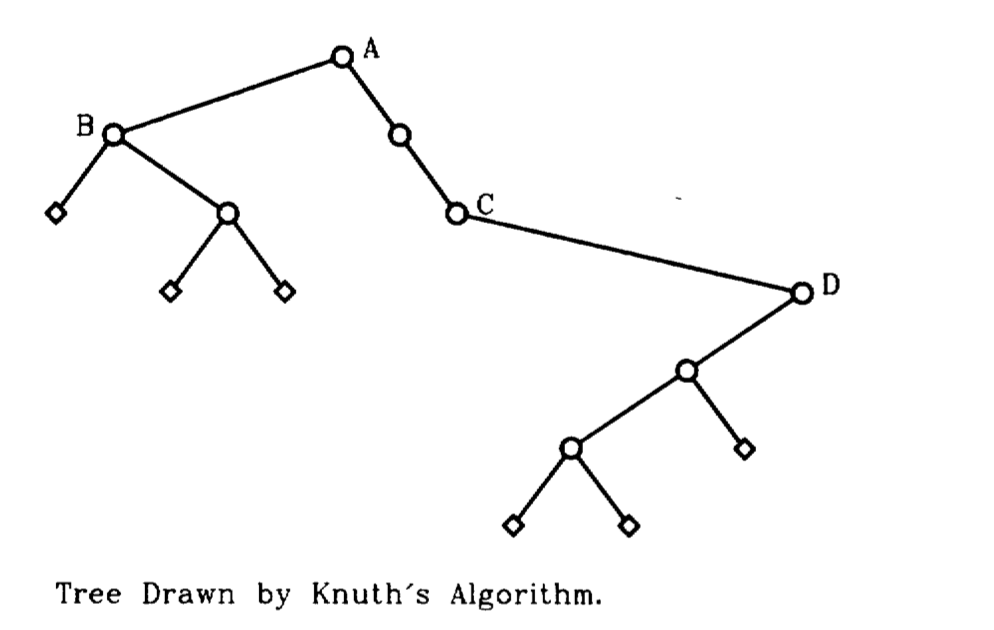
\includegraphics[scale=0.5]{arbreBinaire.png}
    		\end{center}
    	\caption{Arbre binaire dessiné par l'\emph{Algorithme de Knuth}. \cite{article79}}
      \label{fig:arbreBinaire}
    \end{figure}
    \vfill

    L'arbre binaire donné par ce nouvel algorithme respecte bien les contraintes de l'\emph{Esthétique 1} ainsi que de l'\emph{Esthétique 2}, mais notre \emph{Limite physique 1} n'est pas respectée. L'algorithme fait en sorte que lorsqu’un n\oe{}ud occupe une colonne, nul autre n\oe{}ud ne peut occuper cette colonne. Nous obtenons donc une largeur proportionelle au nombre total de n\oe{}uds dans l'arbre.

    Il est alors nécessaire d'utiliser un algorithme différent pour que les conditions de la \emph{Limite Physique} soient respectées.

\newpage
    \subsubsection{Drawings Satisfying the Physical Limit}

    Nous avons vu que l'\emph{Algorithme 1} et l'\emph{Algorithme de Knuth} satisfaisaient chacun des contraintes \emph{Esthétique}. L'idée est ici de fusionner les deux algorithmes pour obtenir un algorithme qui respecte à la fois l'\emph{Esthétique 1}, l'\emph{Esthétique 2} et la \emph{Limite Physique}. L'\emph{Algorithme 3} qui résulte de cette fusion donne des meilleurs arbres que l'\emph{Algorithme 2}, mais ne respecte pas la \emph{Limite Physique} dans toutes les situations.

    \vfill
    \begin{figure}[h]
        \begin{center}
      		\begin{left}
      			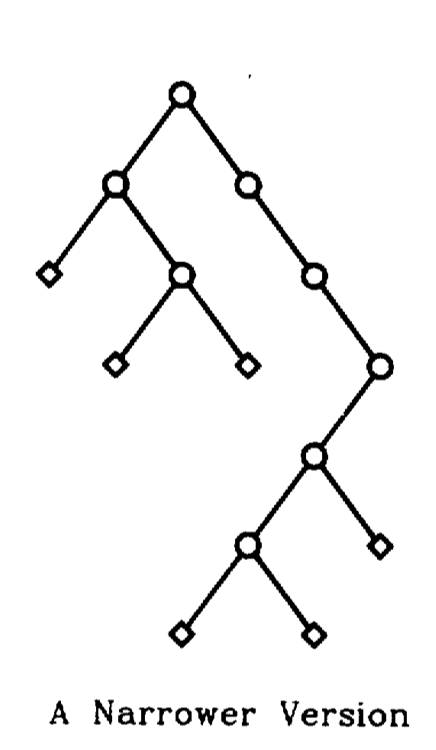
\includegraphics[scale=0.4]{arbreBinaireNarrow.png}
      		\end{left}
          \begin{right}
            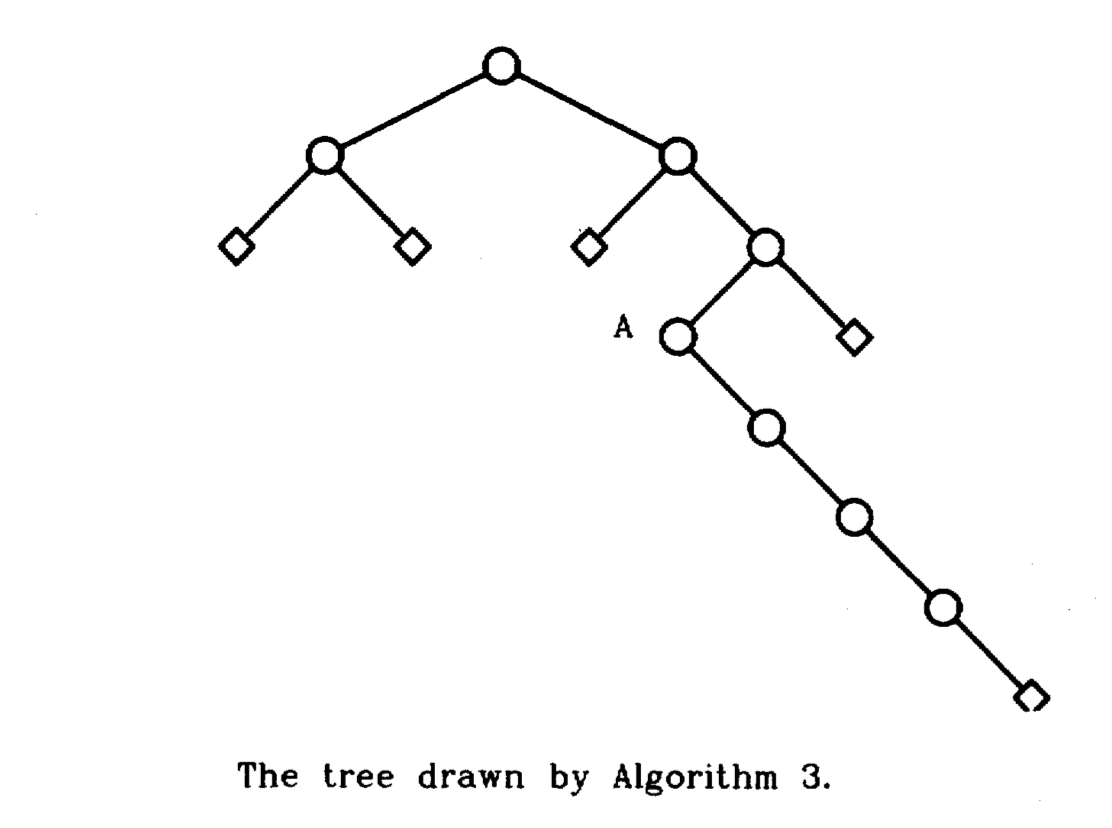
\includegraphics[scale=0.4]{arbre3.png}
          \end{right}
        \end{center}
    	\caption{À gauche l'arbre binaire vu précédement à la Figure \ref{fig:arbreBinaire}; à droite un autre arbre en sortie du même algorithme.  \cite{article79}}
      \label{fig:arbresAlgo3}
    \end{figure}
    \vfill


    L'arbre binaire que nous avons vu à la suite de l'\emph{algorithme de Knuth} est à présent optimal en largeur. Il respecte les contraintes de la \emph{Limite Physique}. Nous constatons que l'arbre qui est à droite, par contre, pourrait être plus optimisé. Il résulte de ce contre exemple que l'\emph{Algorithme 3} doit être modifié afin d'obtenir de meilleurs résultats.

    L'\emph{Algorithme 3} viole en effet la \emph{Limite Physique} car il essaye d'introduire une propriété plus forte de l'\emph{Esthétique 2} : les parents doivent être centrés par rapport à leurs fils.
    Cette \emph{Esthétique 3} inclue les fils directs, mais aussi les fils des fils.

    Face à ce problème, les auteurs de l'article \cite{article79} propose une version modifiée de l'\emph{Algorithme WS}, où l'on privilégie la contrainte de \emph{Limite Physique} plutôt que cette contrainte \emph{Esthétique 3}.

    \vfill
    \begin{figure}[h]
        \begin{center}
      		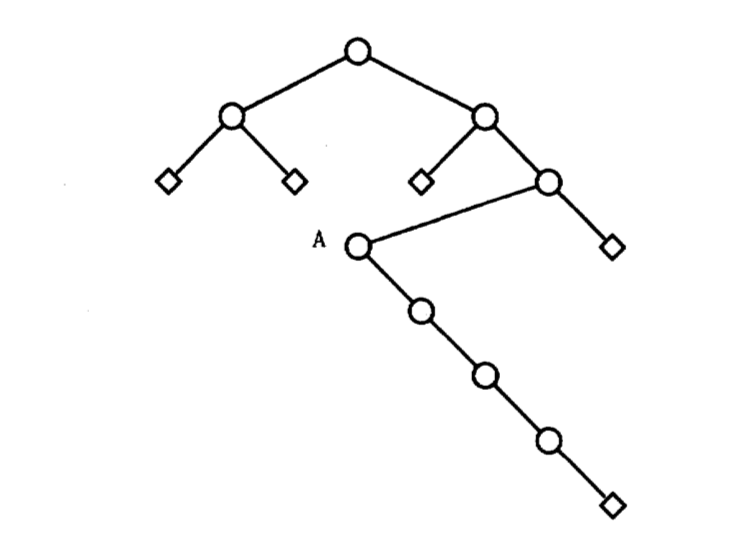
\includegraphics[scale=0.5]{arbreWS.png}
        \end{center}
    	\caption{Arbre de droite de la Figure \ref{fig:arbresAlgo3} après l'\emph{Algorithme WS modifié}. \cite{article79}}
      \label{fig:arbresAlgoWS}
    \end{figure}
    \vfill
    
    L'\emph{Algorithme 3} présenté ne concerne que les arbres binaires mais peut aussi être adapté pour d'autres types d'arbres, en choisissant un moyen de placer les n\oe{}uds parents au-dessus de leurs enfants en tenant compte de leurs nombres ou d'autres spécificités de l'arbre.

\newpage
  \subsection{\emph{Tidier Drawings of Trees}}

  Cet article \cite{article81} reprend les travaux que nous venons de voir. Nous retrouvons donc les trois différentes \emph{Esthétiques} ainsi que la problématique commune de satisfaire à la fois les trois \emph{Esthétiques} et la \emph{Limite Physique}.

  Les auteurs relèvent l'insuffisance de l'\emph{Algorithme WS} pour réaliser des arbres de largeur optimale. Ils notent également la proposition de l'\emph{Algorithme WS modifié} afin de la respecter au détriment de la contrainte \emph{Esthétique 3}. Cependant, ils affirment que les graphes obtenus peuvent être à la fois plus étroits et meilleurs d'un point de vue esthétique (comme nous pouvons le voir à la figure \ref{fig:arbresWSMirror}).

  \vfill
  \begin{figure}[h]
      \begin{center}
        \begin{left}
          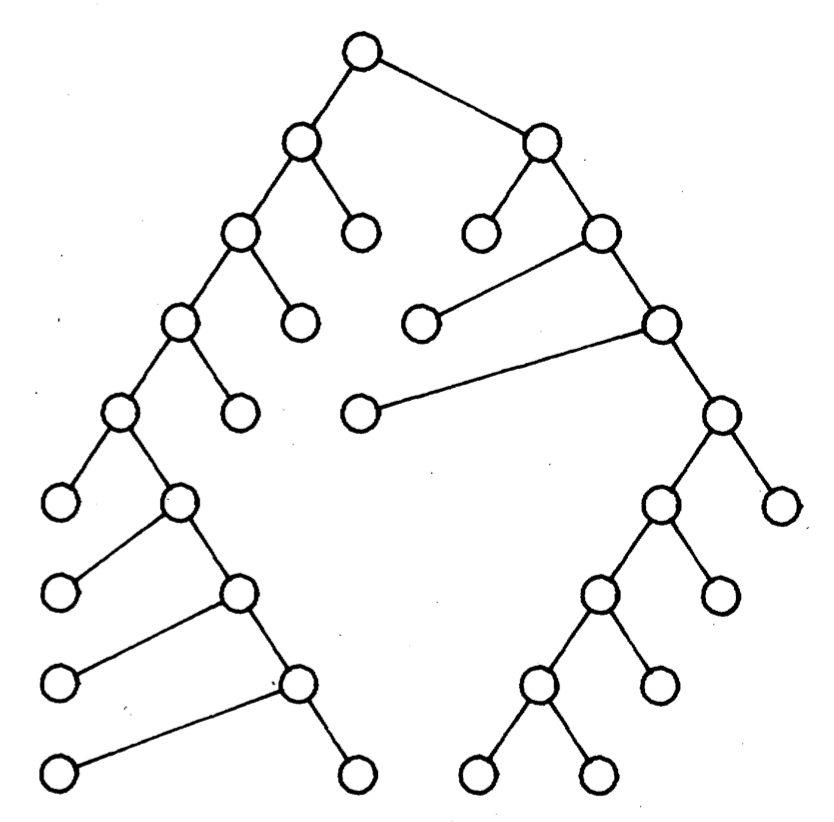
\includegraphics[scale=0.4]{arbreWSM.png}
        \end{left}
        \begin{right}
          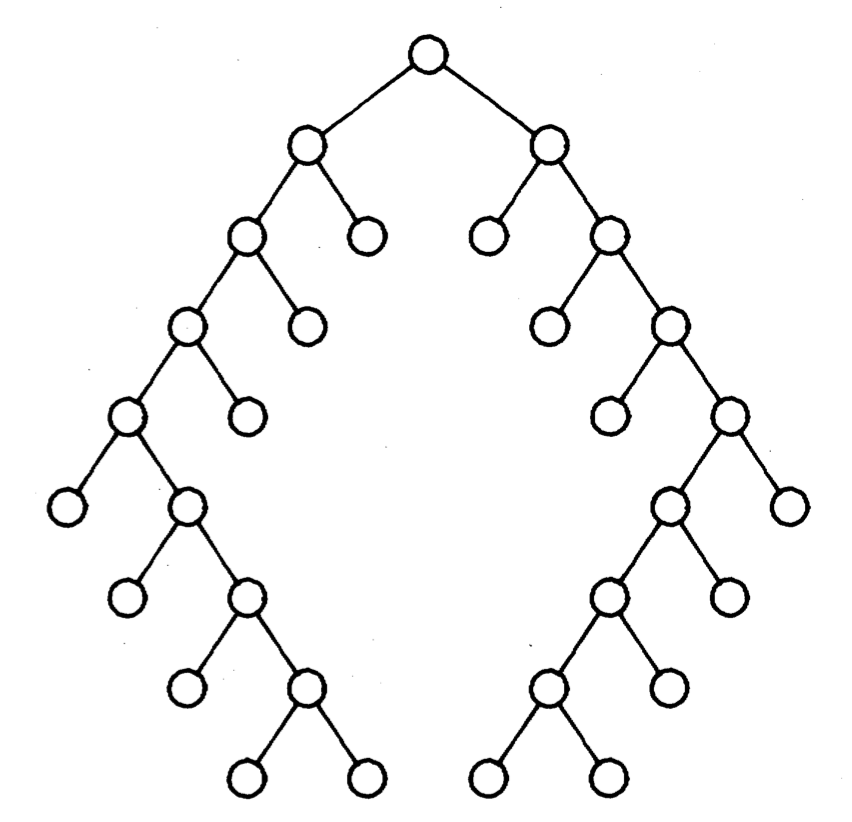
\includegraphics[scale=0.4]{arbreMirror.png}
        \end{right}
      \end{center}
    \caption{À gauche l'arbre binaire avec l'\emph{Algorithme WS modifié}; à droite un arbre plus optimal. \cite{article81}}
    \label{fig:arbresWSMirror}
  \end{figure}
  \vfill

  Pour tenter de parvenir à cette optimisation, une nouvelle contrainte \emph{Esthétique 4} est posée: un arbre et son image miroir doivent être le reflet l'un de l'autre. De plus, un sous-arbre doit être dessiné de la même manière quelle que soit sa position au sein de l'arbre global.

  Il est clairement visible que l'arbre en sortie de l'\emph{Algorithme WS modifié} vu à la Figure \ref{fig:arbresWSMirror} ne respecte pas cette nouvelle contrainte. En la respectant, il devrait ressembler à l'arbre de droite que nous venons de voir sur la même figure.
  
  L'\emph{Algorithme WS modifié} ne peut en effet pas respecter cette contrainte car la forme d'un sous-arbre est modifié en fonction de la position des nodes qui lui sont extérieurs, on peut donc obtenir des sous-arbres à la base symétriques qui sont dessinés assymétriquement.
  
  \vfill
  \begin{figure}[h]
    \begin{center}
        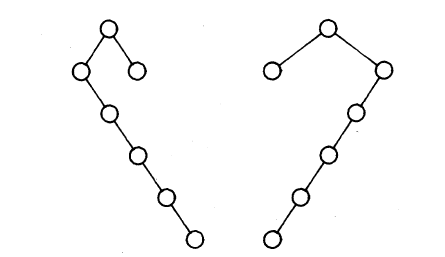
\includegraphics[scale=0.5]{comparArbreMiroirWS.png}
    \end{center}
    \caption{Arbre et son miroir avec l'\emph{Algorithme WS modifié}.
	\cite{article81}}
  \label{fig:arbresAlgoWS}
\end{figure}
\vfill

  Afin de respecter l'\emph{Esthétique 4}, il est nécessaire de sacrifier de la largeur, mais les auteurs considèrent que l'\emph{Esthétique 4} est prioritaire par rapport à la \emph{Limite Physique} pour faciliter la perception humaine.
  
  L'idée de l'algorithme proposé, l'\emph{Algorithme TR}, est de générer les sous-arbres d'un même n\oe{}ud de manière séparée, puis de les placer les plus proches possible.
  Ceci est d'abord réalisé par un parcours postfixe, en superposant les arbres et en les déplaçant jusqu'à ce que les arbres ne se chevauchent à aucun niveau de profondeur, avec une distance minimale incompressible définie. Une fois ces positions connues, il suffit de faire un parcours préfixe de l'arbre, en donnant des positions absolues aux n\oe{}uds.
  
  Cet algorithme respecte à la fois les contraintes d'\emph{Esthétique 1}, \emph{Esthétique 2}, \emph{Esthétique 3}, mais en plus l'\emph{Esthétique 4} définie précédemment.
  
  
  \subsubsection{Generalization to m-ary trees and forests}
  L'\emph{Algorithme TR} peut facilement être adapté pour des arbres n-aires, sans en affecter les performances, en effectuant n-1 opérations de séparation des sous-arbres.
  Pour les forêts, cela dépend de la représentation utilisée, mais reste possible et est détaillé dans un autre article.
  
  \subsection{\emph{A Node-Positioning Algorithm for General Trees}}
  
  L'article \cite{article90} s'intéresse au cas général des arbres n-aires, en gardant comme objectif le respect des contraintes définies dans les précédents articles, sauf l'\emph{Esthétique 2}, qui n'est pas pertinente dans les cas où les n\oe{}uds ont plus de deux fils.
  L'\emph{Esthétique 4}, définie plus tôt, est d'ailleurs renforcée en imposant également que des petits sous-arbres ne soient pas arbitraitement positionnés lorsque proches d'autres sous-arbres plus grands.
  Ainsi, des petits sous-arbres aux extrêmes gauche et droite devraient être placés de manière adjacente à leurs sous-arbres voisins plus grands.
  
  Il est admis qu'on ne cherche que la position en $x$ des n\oe{}uds, la position en $y$ étant déterminée par la hauteur dans l'arbre.
  
  L'algorithme proposé réalise deux parcours de l'arbre. Premièrement, on parcourt l'arbre en assignant une valeur en $x$ temporaire à chaque n\oe{}ud ainsi qu'en remplissant un champ particulier qui servira à décaler ses noeuds au second parcours. Ce premier parcours est réalisé de la même manière que dans l'article \cite{article81}, avec un parcours postfixe qui décale les sous-arbres des n\oe{}uds de manière à respecter à tous les niveaux de profondeur un écartement défini. On peut noter qu'il n'y a pas de mécanisme pour rapprocher les sous-arbres alors qu'on pourrait à une itération ne pas avoir à écarter les sous-arbres, dans le cas d'un sous-arbre gauche très écarté vers la gauche par exemple, mais que l'on ne rapproche pas pour autant, alors qu'il pourrait être très éloigné d'un grand sous-arbre droit. Cet agglutinement est d'ailleurs selon les auteurs le défaut des algorithmes précédents (articles \cite{article79}, et \cite{article81}).
  La correction proposée est d'utiliser un modificateur de position pour déplacer les sous-arbres, et dans ce cas précis les rapprocher lorsque c'est possible.
  
  Le second parcours permet d'attribuer la coordonnée en $x$ définitive grâce à ce modificateur présents sur les n\oe{}uds.
  
   \vfill
  \begin{figure}[h]
    \begin{center}
        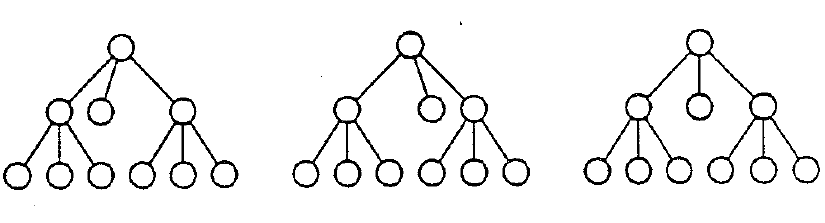
\includegraphics[scale=0.5]{arbreWalker.png}
    \end{center}
    \caption{Arbres montrant l'effet observé d'agglutinement à gauche, à droite, puis le résultat idéal.
	\cite{article90}}
  \label{fig:arbresAlgoWS}
\end{figure}
\vfill
  
  
  \subsection{\emph{Improving Walker’s Algorithm to Run in Linear Time}}
  
  

\newpage
\section{Implémentation des algorithmes}

Suite à la lecture et à l'analyse des articles, il nous faut maintenant implémenter les algorithmes que nous venons de brièvement présenter. Il va sans dire que nous n'allons pas implémenter la totalité des algorithmes, mais seulement le deux qui nous semblent \emph{clés} dans l'évolution chronologique de l'optimisation d'arbre.

Implémenter les algorithmes en Python n'était pas chose simple, il nous a fallu comprendre la version des algorithmes tantôt en \emph{Pascal}, tantôt en \emph{Pseudo-code}. Le fait que les articles datent de quelques années (voir de quelques décennies pour certain) nous a posé problème. En effet, nous nous sommes interrogé sur la logique algorithmique de certains codes, notamment l'\emph{Algorithme de Walker} de l'article \cite{article90}. De plus, la clarté des paragraphes explicatifs des algorithmes laissant à désirer, la tâche de compréhension et retranscription de certaines fonctions n'a pas été facile. Nous avons également constaté que certaines fonctions (et non les plus triviales) ne sont pas définies bien qu'utilisées dans les algorithmes. 

Les algorithmes que nous avons trouvés les plus pertinents à implémenter sont: celui de \emph{Walker} décrit dans l'article \cite{article90} et celui décrit dans l'article \cite{article02} qui est une modification de l'\emph{Algorithme de Walker}.

\subsection{Implémentation \emph{Python} de l'\emph{Algorithme de Walker} \cite{article90}}

\subsection{Implémentation \emph{Python} de l'\emph{Algorithme de Walker} amélioré \cite{article02}}

\subsection{Différences Algorithmiques}


\newpage
\section{Étude empirique des algorithmes}

L'implémentation en \emph{Python} des deux algorithmes étant réalisée, il est questions maintenant d'étudier leur comportement sur des jeux de données. Nous allons pouvoir ainsi comparer les résultats entre la version initiale de  l'\emph{Algorithme de Walker} et sa version modifiée dans l'article \cite{article02}.

Nous profiterons de cette étude empirique comparative de nos deux algorithmes pour comparer également les résultats obtenus entre notre \emph{Algorithme de Walker} amélioré et entre celui qui est disponible dans \emph{Tulip} qui se nomme \emph{Improved Walker}


\newpage
\section{Conclusion}




\newpage
\medskip

\begin{thebibliography}{10}

\bibitem{article79}
C. Wetherell and A. Shannon. Tidy Drawings of Trees. \textit{IEEE transactions on Software Engineering} SE-5, 5 (septembre 1979) p514-520.

\bibitem{article81}
E. Reingold and J. Tilford. Tidier Drawings of Trees. \textit{IEEE Transactions on Software Engineering} SE-7, 2 (mars 1981) p223-228.

\bibitem{article90}
J. Walker II. A Node-Positioning Algorithm for General Trees. \textit{Software – Practice and Experience} SE-20, 2 (1990) p685–705.

\bibitem{article02}
C. Buchheim, M. Jünger and S. Leipert. Improving Walker’s Algorithm to Run in Linear Time. Technical Report zaik2002-431, ZAIK, Universität zu Köln, (2002) p344-352.

\end{thebibliography}

\end{document}
